%! Author = melek
%! Date = 22.01.2023

% Preamble
\documentclass[11pt]{article}

% Packages
\usepackage{amsmath}
\usepackage{graphicx}
\graphicspath{ {../images/} }

\title{Assignment 3: Q-Learning and Actor-Critic Algorithms}
\author{huseyinabanox@gmail.com}
\date{January 2023}

% Document
\begin{document}

    \maketitle

    \section{Part 1: Q-Learning}

    \subsection*{Question 1: basic Q-learning performance (DQN)}

    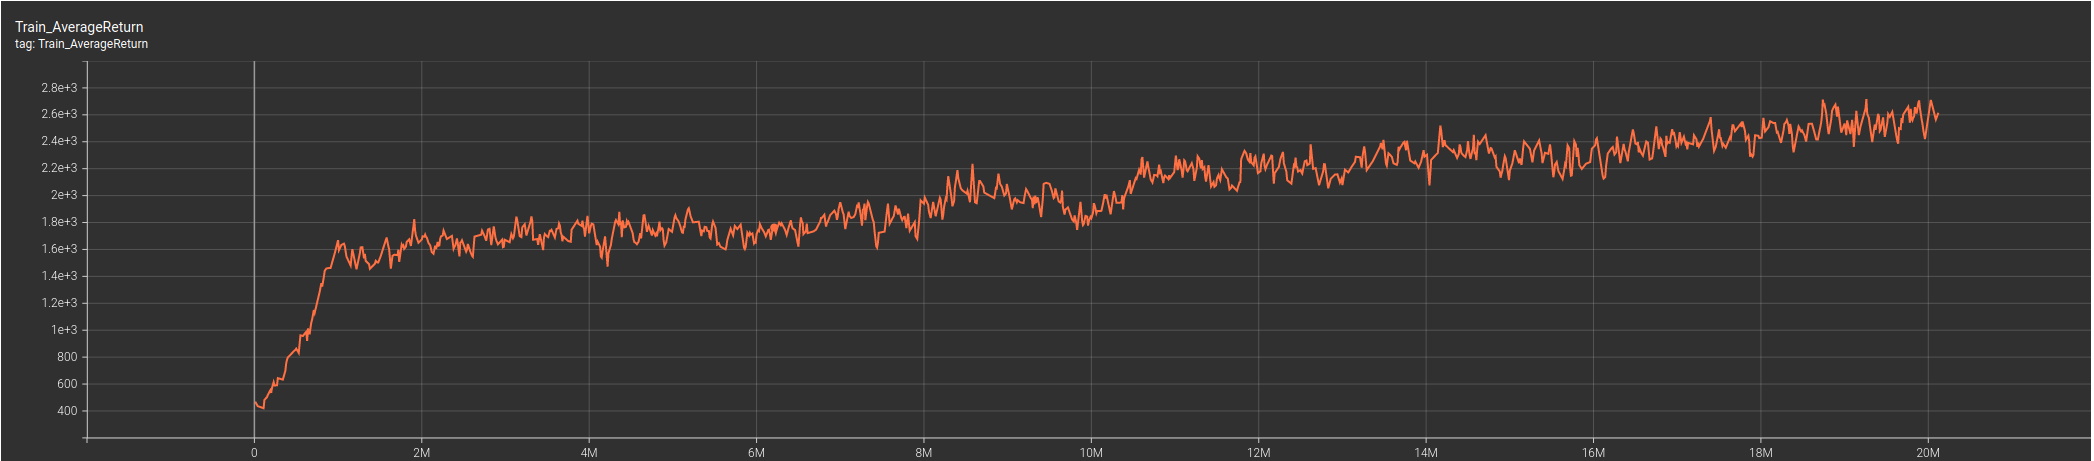
\includegraphics[scale=0.8]{q1/packman-20M}

    After 20M iterations the learning curve looks like above.
    It is taken from tensorboard.
    Relevant log files can be found under data folder.

    Double Q network obtains better returns, as expected.

    \subsection*{Question 2: double Q-learning (DDQN)}

    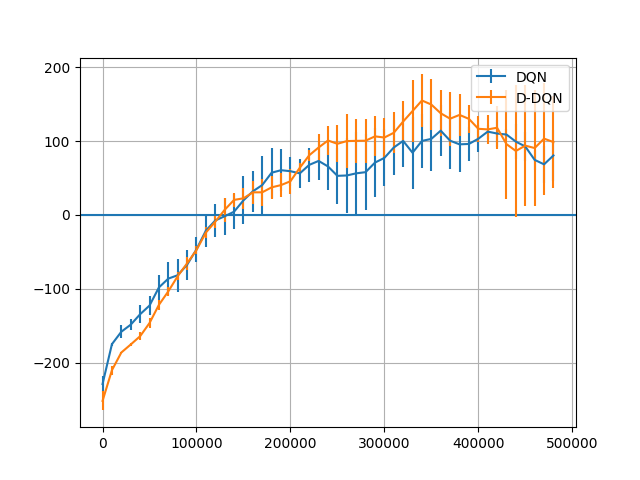
\includegraphics[scale=0.8]{q2/q2}

    LunarLander-v3 environment is used for 3 seeds per configuration e.g. DQN vs D-DQN as stated in the question.
    Different seed results are averaged and the plot above is generated.
    combine\_results\_q2.py file is used to combine results.

    \subsection*{Question 3: experimenting with hyperparameters}

    TODO: solve this question

    \section{Part 2: Actor-Critic}

    \subsection*{Question 4: Sanity check with Cartpole}

    Actor critic algorithm is tested in cartpole environment.
    Different target update parameters and gradient steps parameters are tried.

    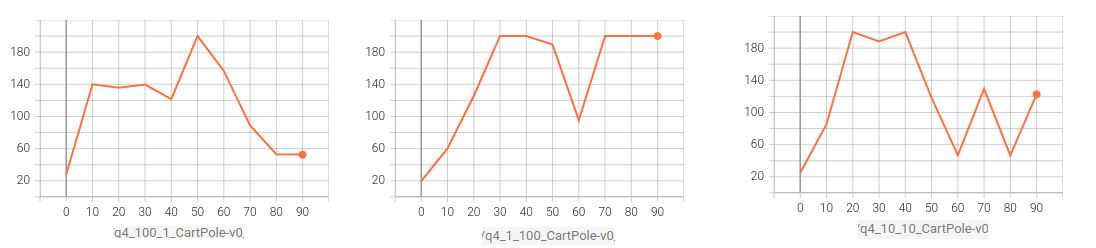
\includegraphics[scale=1.5]{q4/q4}.

    Subtitles show the used parameters.

    Best performance is obtained when both parameters are set to 10.
    If target update is set to 1 and gradient steps are set to 100, learning seems to be more stable.
    This results shows the importance of gradient steps.

    \subsection*{Question 5: Run actor-critic with more difficult tasks}

    Best results are obtained when both parameters are set to 10.

    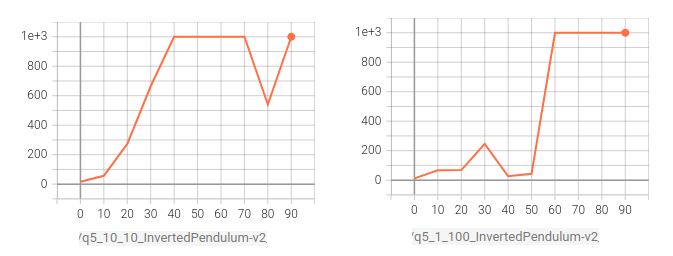
\includegraphics[scale=2]{q5/q5_inverted_pendulum}.

    After 100 iterations, InvertedPendulum return is around 1000, as expected.
    After 20 iterations, InvertedPendulum return should is above 100, as expected.

    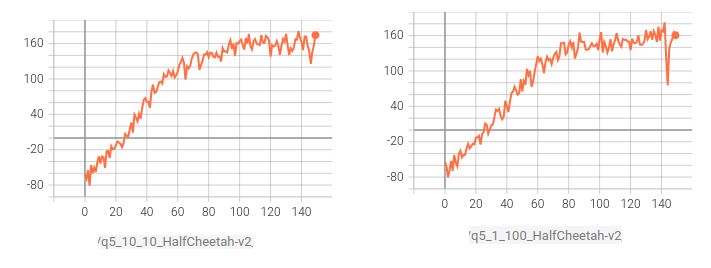
\includegraphics[scale=2]{q5/q5_half_cheetah}.

    After 150 iterations, HalfCheetah return is around 150, as expected.
    After 20 iterations, HalfCheetah return is above -40, as expected.

    \section{Part 3: Soft Actor-Critic}

    \subsection*{Question 6: Run soft actor-critic more difficult tasks}

    Actor updates and critic updates are set to 10.

    After 20000 steps, InvertedPendulum return is expected to reach 1000.
    Actually it is reached after 9k steps.

    \subsection*{Question 6: Run soft actor-critic more difficult tasks}

    The same parameters are used as stated in the question.
    Additionally \textless num\_critic\_updates\_pe\_agent\_update\textgreater and \textless num\_acto\_updates\_per\_agent\_update\textgreater parameters are set to 10.

    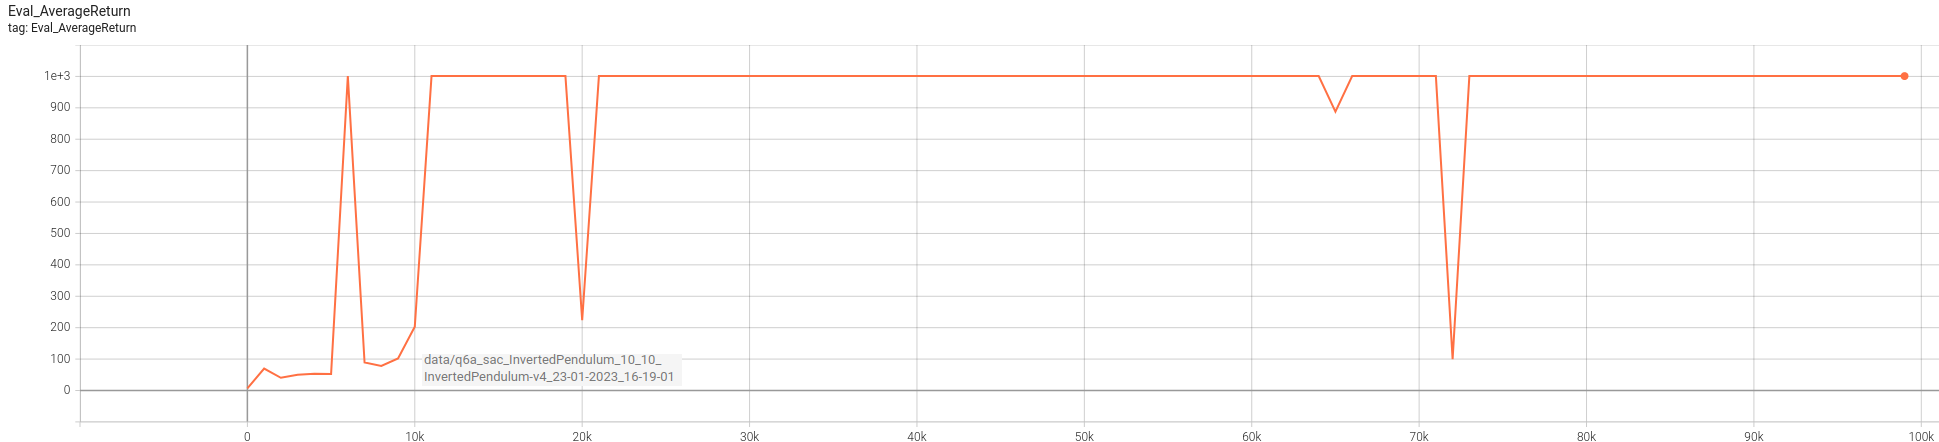
\includegraphics[scale=0.66]{q6/inverted_pendulum}.

    After 10000 steps, InvertedPendulum return is expected to be near or above 100.
    After 20000 steps, InvertedPendulum return is expected to reach 1000.
    Our implementation reaches 1000 before 10K steps and stabilizes around 1000 after 10K steps.

    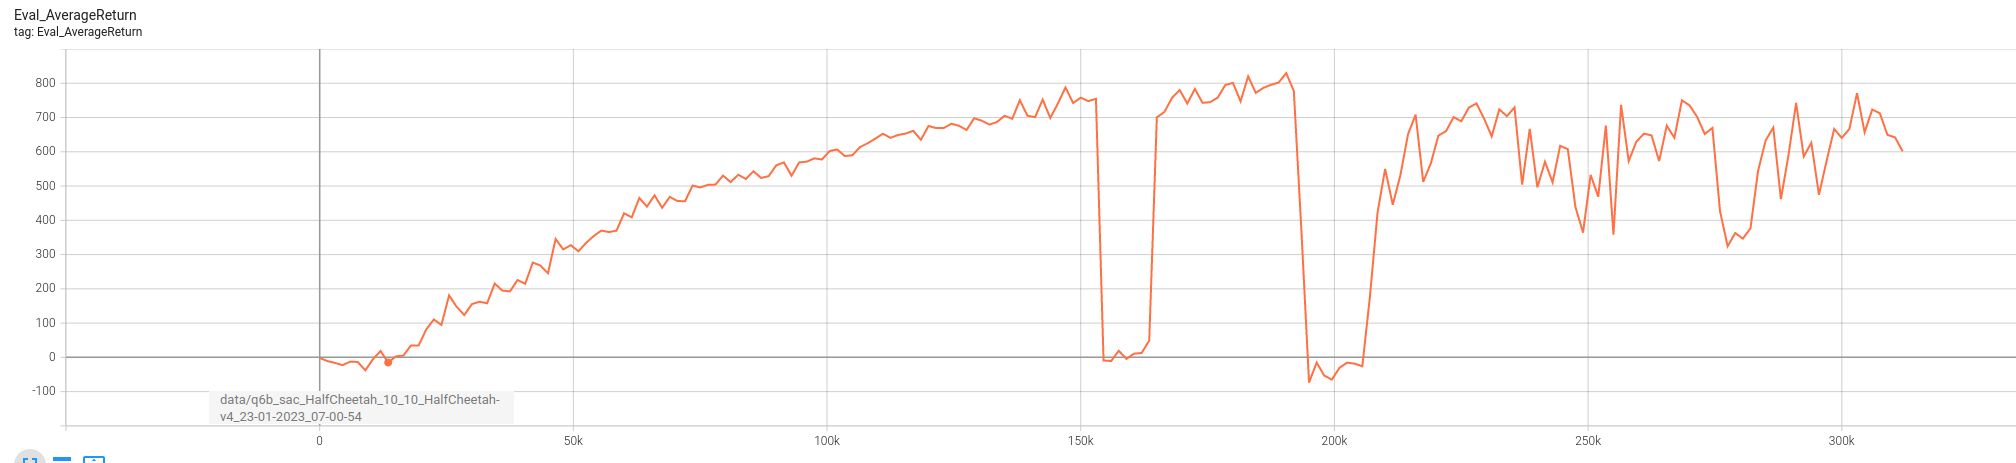
\includegraphics[scale=0.66]{q6/halfcheatah}.

    After 10000 steps, HalfCheetah return is expected to be above -40 (trending toward positive).
    After 50000 steps, HalfCheetah return should be around 200.
    Our implementation return is close to zero at 10K steps and is above 300 after 50K steps.




\end{document}